% @Author: luis
% @Date:   2016-02-20 12:42:09
% @Last Modified by:   luis
% @Last Modified time: 2016-03-11 18:53:27

% @Author: Luis Perez
% @Date:   2016-02-02 21:09:55
% @Last Modified by:   luis
% @Last Modified time: 2016-02-19 17:47:15

\documentclass[12pt]{article}
\usepackage{latexsym}
\usepackage{fancyhdr}
\usepackage{amssymb,amsmath,amsthm}
\usepackage[pdftex]{graphicx}
\usepackage{pdfpages}
\usepackage{hyperref}
\usepackage[margin=1in]{geometry}


% Create answer counter to keep track of seperate responses
\newcounter{AnswerCounter}
\newcounter{SubAnswerCounter}
\newcounter{SubSubAnswerCounter}
\setcounter{AnswerCounter}{1}
\setcounter{SubAnswerCounter}{1}
\setcounter{SubSubAnswerCounter}{1}

% Create answer environment which uses counter
\newenvironment{answer}[0]{
  \setcounter{SubAnswerCounter}{1}
  \bigskip
  \textbf{Solution \arabic{AnswerCounter}}
  \\
  \begin{small}
}{
  \end{small}
  \stepcounter{AnswerCounter}
}

\newenvironment{subanswer}[0]{
  \setcounter{SubSubAnswerCounter}{1}
  (\alph{SubAnswerCounter})
}{
 \bigskip
  \stepcounter{SubAnswerCounter}
}

\newenvironment{subsubanswer}[0]{
  \hspace{0.25in}[\roman{SubSubAnswerCounter}]
}{
 \bigskip
  \stepcounter{SubSubAnswerCounter}
}

% Allows easy use of vectors
\newcommand{\vect}[1]{\vec{\boldsymbol{#1}}}
\newcommand{\deln}[3]{\frac{\partial^{#3} #1}{\partial #2^{#3}}}
\newcommand{\del}[2]{\frac{\partial#1}{\partial #2}}
\newcommand{\bra}[1]{\langle {#1} |}
\newcommand{\ket}[1]{| {#1} \rangle}
\newcommand{\braket}[3]{\langle {#1} | {#2} | {#3} \rangle}



% Custom Header information on each page
\pagestyle{fancy}
\lhead{HUID: 70871564}
\rhead{Luis Perez - \thepage}
\renewcommand{\headrulewidth}{0.1pt}
\renewcommand{\footrulewidth}{0.1pt}

\newcommand{\horrule}[1]{\rule{\linewidth}{#1}}   % Horizontal rule
\title{
    % \vspace{-1in}
    \usefont{OT1}{bch}{b}{n}
    \normalfont \normalsize \textsc{Harvard University} \\ [25pt]
    \horrule{0.5pt} \\[0.4cm]
    \huge Physics 143a: Quantum Mechanics I \\ [20pt]
    \normalfont \normalsize Problem Set 4
    \horrule{2pt} \\[0.5cm]
}
\author{
    \normalfont                 \normalsize
        Luis Antonio Perez\\[-3pt]    \normalsize
}
\date{\today}

\begin{document}
\maketitle
\pagebreak

\begin{answer}
We use raising and lowering operators to calculate the following for the harmonic oscillator system.
\begin{subanswer}
We calculate the uncertainty in $x$ for a system in an energy eigenstates of the harmonic oscillator.
\begin{align*}
\Delta x &= \sqrt{\langle n | x^2 | n \rangle - \langle n | x | n\rangle} \\
&= \sqrt{\frac{\hbar}{2mw_0} [\langle n | [a^\dag + a]^2 | n \rangle  - \langle n | a^\dag + a | n \rangle^2]} \\
&= \sqrt{\frac{\hbar}{2mw_0} \left[ \langle n | a^\dag a^\dag | n \rangle + \langle n | a^\dag a | n \rangle  + \langle n | aa^\dag | n \rangle + \langle n | aa | n \rangle - (\langle n | a^\dag | n \rangle + \langle n | a | n \rangle)^2 \right]} \\
&= \sqrt{\frac{\hbar}{2mw_0} \left[ \sqrt{(n+1)(n+2)}\langle n | n + 2 \rangle +  n\langle n | n \rangle  + (n+1)\langle n | n \rangle + \sqrt{n(n-1)}\langle n | n - 2 \rangle - (\sqrt{n+1}\langle n | | n + 1 \rangle + \sqrt{n} \langle n| n -1\rangle \right]})^2 \\
&= \sqrt{\frac{\hbar}{2mw_0}(2n + 1)}
\end{align*}
where the simplifications in the last line occur because of orthonormality when using a single raising or lowering operator.
\end{subanswer}

\begin{subanswer}
We calculate the uncertainty in $p$ for a system in an energy eigenstates of the harmonic oscillator.
\begin{align*}
\Delta p &= \sqrt{\langle n | p^2 | n \rangle - \langle n | p | n\rangle} \\
&= \sqrt{-\frac{m\hbar w_0}{2} [\langle n | [a^\dag - a]^2 | n \rangle  - \langle n | a^\dag - a | n \rangle^2]} \\
&= \sqrt{-\frac{m\hbar w_0}{2} \left[ \langle n | a^\dag a^\dag | n \rangle - \langle n | a^\dag a | n \rangle  - \langle n | aa^\dag | n \rangle + \langle n | aa | n \rangle - (\langle n | a^\dag | n \rangle - \langle n | a | n \rangle)^2 \right]} \\
&= \sqrt{\frac{m\hbar w_0}{2}(2n + 1)}
\end{align*}
where the simplifications in the last line follows directly form the simplifications performed above.
\end{subanswer}

\begin{subanswer}
We now calculate the product in the uncertainties of $x$ and $p$ in the energy eigenstates.
\begin{align*}
\Delta p \Delta q &= (2n+1)\sqrt{\frac{m\hbar^2 w_0}{4 m w_0}} \\
&= (2n+1)\frac{\hbar}{2}
\end{align*}
and comparing this to that predicted by the generalized uncertainty principle:
\begin{align*}
\Delta x \Delta p \geq \frac{1}{2} [x,p] = \frac{\hbar}{2}
\end{align*}
Note that the computed values agrees with the prediction form the generalized uncertainity principle because $n > 0$ implies that $\delta p \Delta q \geq \frac{\hbar}{2}$.
\end{subanswer}

\begin{subanswer}
Note that we can solve for $\tilde{x}$ and $\tilde{p}$ from the given:
\begin{align*}
x &= \sqrt{\frac{2\hbar}{mw_0}} \tilde{x} \\
p &= \sqrt{2m\hbar w_0} \tilde{p}
\end{align*}
as follows:
\begin{align*}
\tilde{x} &= \sqrt{\frac{mw_0}{2\hbar}}x \\
\tilde{p} &= \sqrt{\frac{1}{2m\hbar w_0}} p
\end{align*}

With the above, we can rewrite the Hamiltonian and calculate the uncertainties in $\tilde{x}$ and $\tilde{p}$. We have:
\begin{align*}
H &= \frac{p^2}{2m} + \frac{1}{2}mw_0^2x^2 \\
&= \frac{2m\hbar w_0}{2m}\tilde{p}^2 + \frac{1}{2}mw_0^2\left(\frac{2\hbar}{mw_0} \tilde{x}^2\right) \\
&= \hbar w_0 \tilde{p}^2 + \hbar w_0 \tilde{x}^2 \\
&= \hbar w_0 [ \tilde{p}^2 + \tilde{x}^2]
\end{align*}
Now we compute the uncertainties in $\tilde{x}$ and $\tilde{p}$:
\begin{align*}
\Delta \tilde{x} &= \sqrt{ \langle n | \tilde{x}^2 | n \rangle - \langle n | \tilde{x} | n \rangle ^2} \\
&= \sqrt{\frac{mw_0}{2 \hbar}}\Delta x \\
&= \frac{1}{2}\sqrt{2n + 1}
\end{align*}
and
\begin{align*}
\Delta \tilde{p} &= \sqrt{ \langle n | \tilde{p}^2 | n \rangle - \langle n | \tilde{p} | n \rangle ^2} \\
&= \sqrt{\frac{1}{2 m \hbar w_0}} \Delta p \\
&= \frac{1}{2}\sqrt{2n + 1}
\end{align*}
\end{subanswer}

\begin{subanswer}
The plot is in Figure \ref{fig:uncertainty_principle}. Note that is has additional lines that we will add as the assignment progresses. The line along the furthest down is indicative of the region specified by the general uncertainty principle:
\begin{align*}
\Delta \tilde{x} \Delta \tilde{p} &\geq \frac{1}{2} |[\tilde{x}, \tilde{p}]| \\
&= \frac{1}{2}\sqrt{\frac{mw_0}{2\hbar}\frac{1}{2m\hbar w_0}}|[x,p] |\\
&= \frac{1}{4\hbar} |[x,p]| \\
&= \frac{1}{4}
\end{align*}
and for each energy eigenstate we have:
\begin{align*}
\Delta \tilde{x} \Delta \tilde{p} &= \frac{1}{4}(2n + 1)
\end{align*}
giving us for $n \in \{0,1,2,3\}$:
\begin{align*}
\Delta \tilde{x} \Delta \tilde{p} &= \frac{1}{4} \\
\Delta \tilde{x} \Delta \tilde{p} &= \frac{3}{4} \\
\Delta \tilde{x} \Delta \tilde{p} &= \frac{5}{4} \\
\Delta \tilde{x} \Delta \tilde{p} &= \frac{7}{4}
\end{align*}
\begin{figure}
\centering
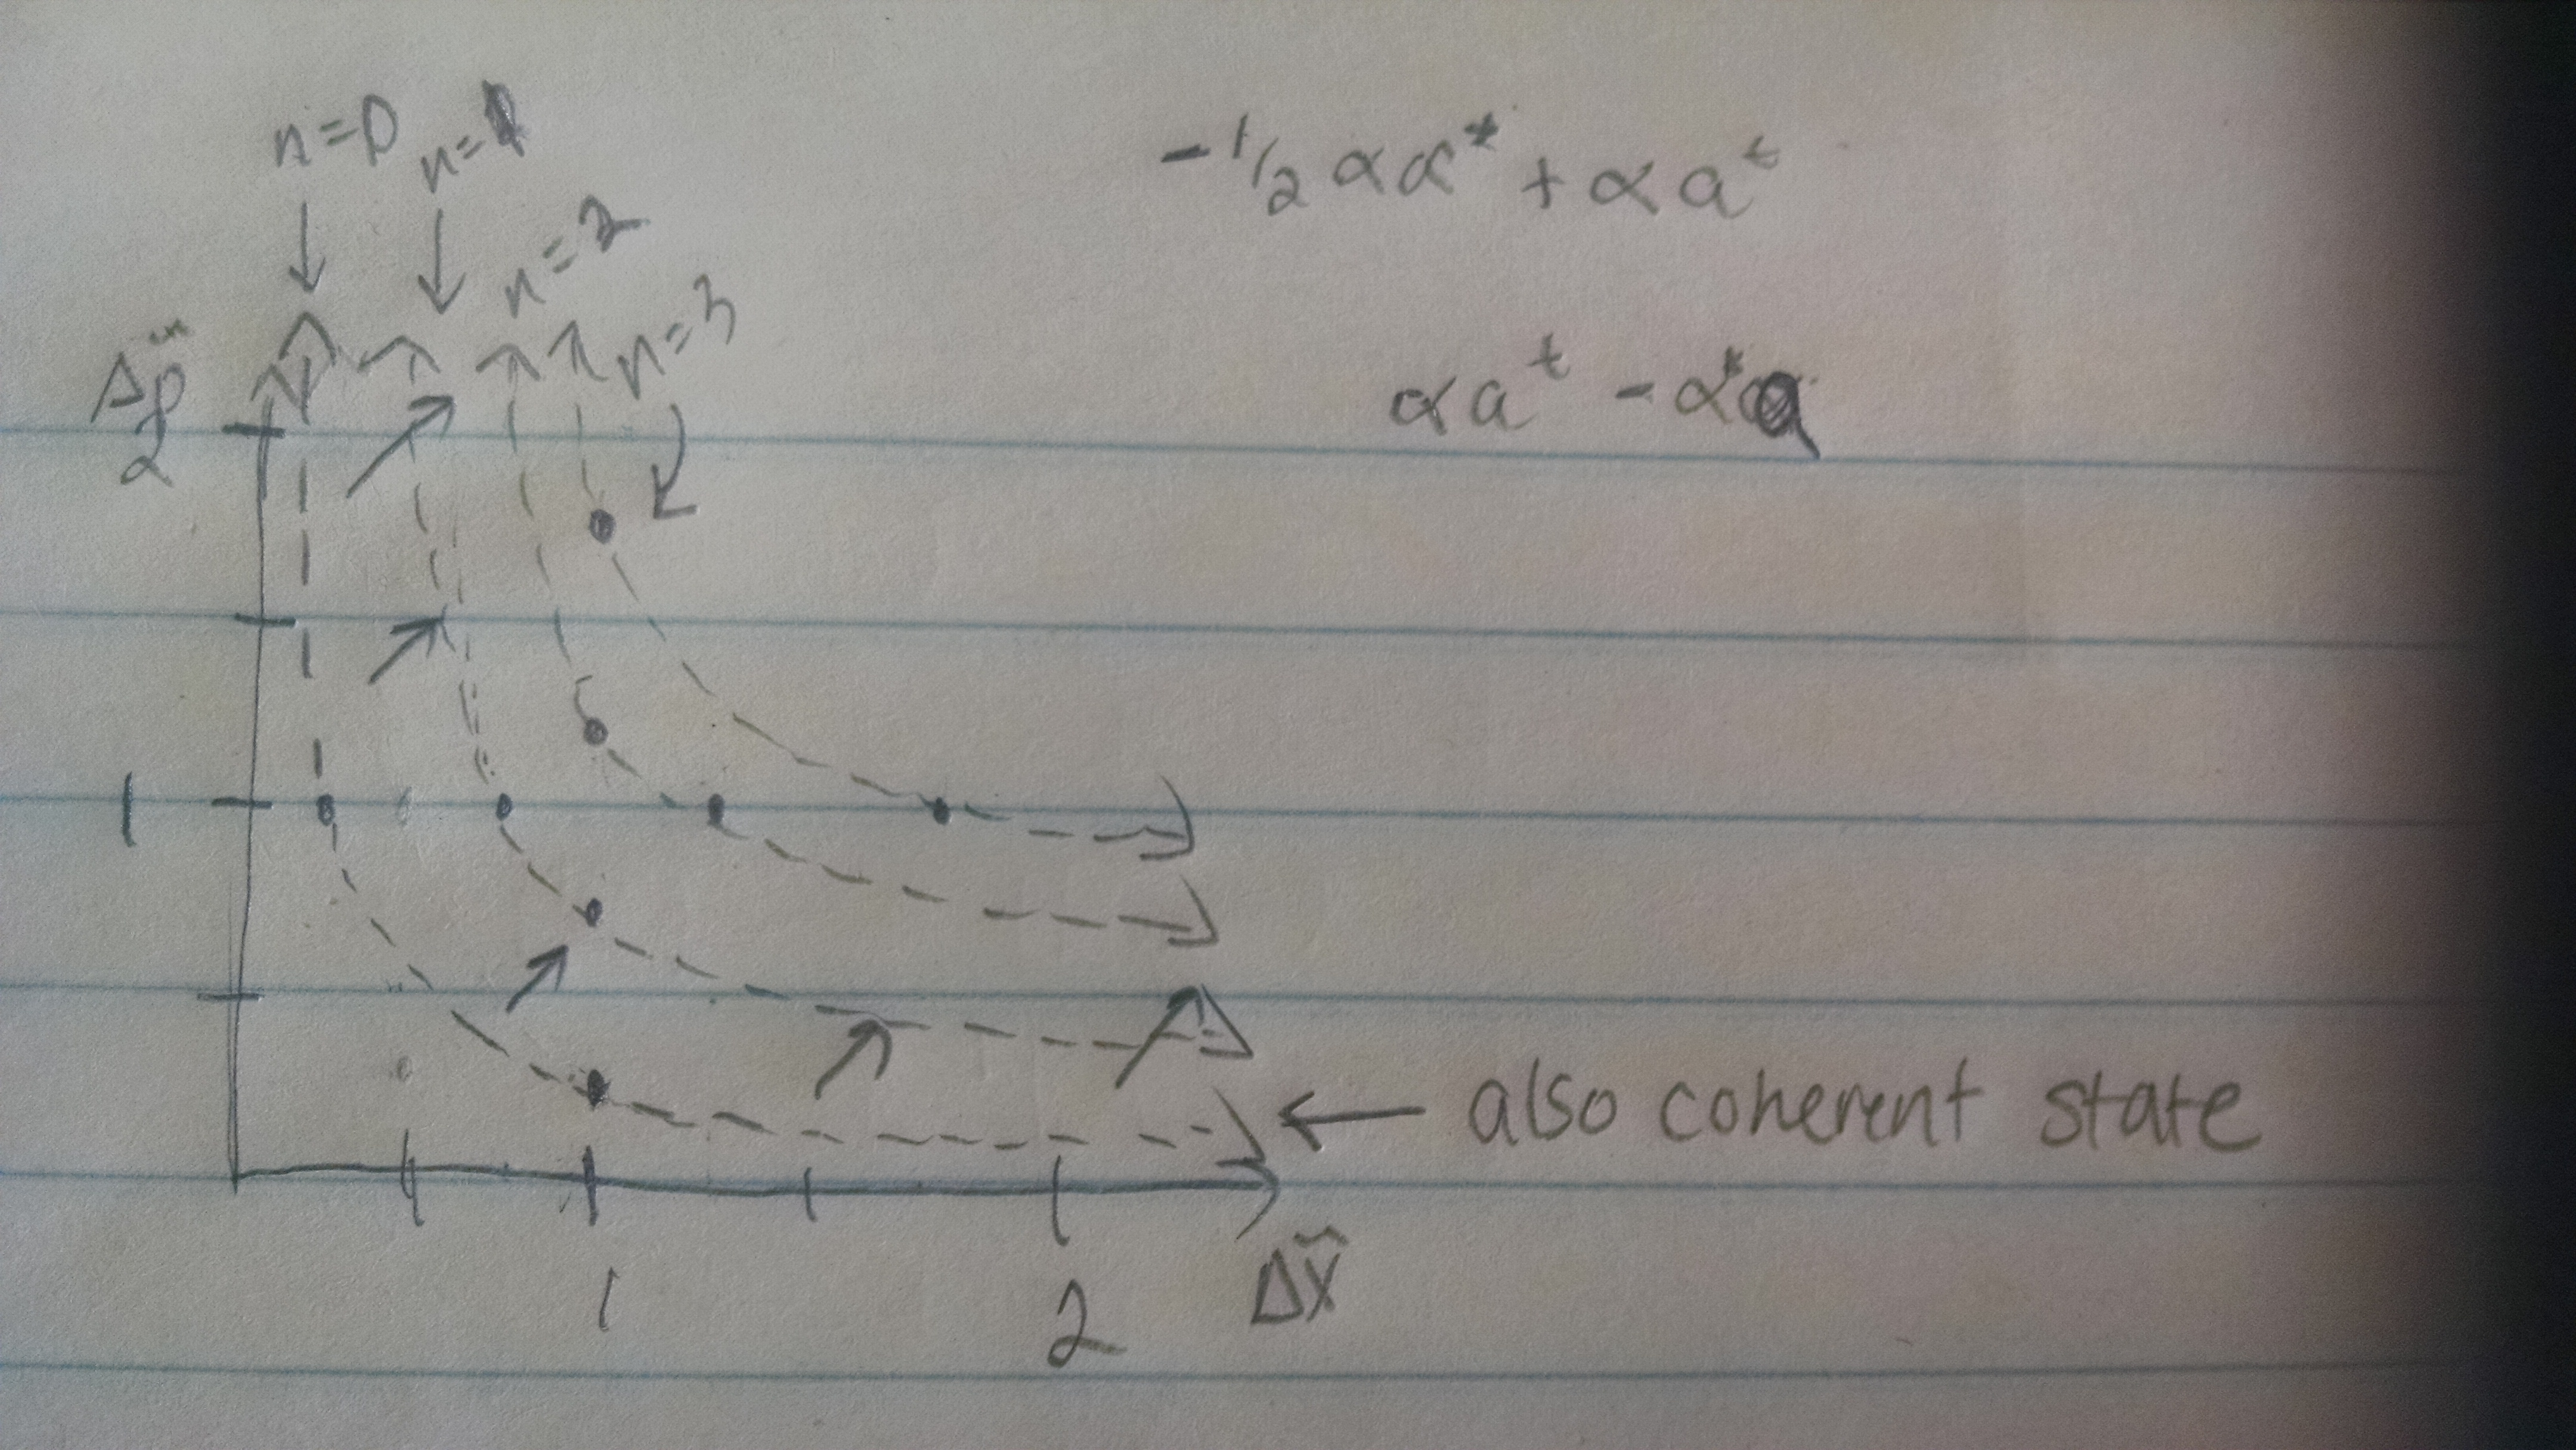
\includegraphics[scale=0.1]{graphs.jpg}
\caption{Uncertainty Principle Graph}
\label{fig:uncertainty_principle}
\end{figure}
\end{subanswer}
\end{answer}

\begin{answer}
We now study the coherent state of the harmonic oscillator, $|\alpha \rangle$ such that $a|\alpha \rangle = \alpha | \alpha \rangle$ where $a$ is the lowering operator.

\begin{subanswer}
We wish to find $\ket{\alpha}$. Since we know that $\ket{n}$ span the space, we can write:
$$
\ket{\alpha} = \sum_{n=1}^{\infty} c_ne^{i\delta_n}\ket{n}
$$
where, for simplicity, we assume $c_n$ real and $\delta_n = 0$ (ie, all of the energy eigenstates are in the same phase). Given that we want the eigenvalue of $\ket{\alpha}$ to be $\alpha$, we have that the following condition must hold:
\begin{align*}
a\ket{\alpha} &= \alpha\ket{\alpha}\\
\implies \sum_{n=0}^{\infty} c_{n}[a\ket{n}] &= \sum_{n=0}^{\infty} \alpha c_n e^{i\delta_n}\ket{n} \\
\implies \sum_{n=0}^{\infty} c_{n+1}\sqrt{n+1}\ket{n} &= \sum_{n=0}^{\infty} \alpha c_n \ket{n} \\
\implies c_{n+1} = \frac{\alpha c_n}{\sqrt{n+1}} \\
\implies c_{n} = \frac{\alpha c_{n-1}}{\sqrt{n}} \\
\implies c_{n} = \frac{\alpha^n c_0}{\sqrt{n!}}
\end{align*}
Therefore, if we let $\ket{\alpha} = \sum_{n=0}^{\infty} c_n \ket{n}$ where $c_n =  \frac{\alpha^n c_0}{\sqrt{n!}}$for some constant $c_0$, we will have a coherent state. To simplify calculations further, we pick $c_0$ to be real which implies $c_n $ is real $\forall n$. We leave out phase factors and dependence on time. We can write the final form as:
$$
\ket{\alpha} = c_0\sum_{n=0}^{\infty} \frac{\alpha^n}{\sqrt{n!}}\ket{n}
$$
\end{subanswer}

\begin{subanswer}
When normalizing the coherent states, we just need to find the $c_0$ such that we have normalized coefficients. We require that:
\begin{align*}
\sum_{n=0}^{\infty} |c_n|^2 &= 1 \\
\implies  \sum_{n=0}^{\infty} \frac{|\alpha|^{2n}|c_0|^2}{n!} &= 1 \\
\implies |c_0|^2 \sum_{n=0}\frac{|\alpha|^{2n}}{n!} &= 1 \\
\implies |c_0|^2 e^{|\alpha|^2} &= 1 \\
\implies |c_0| &= e^{-\frac{|\alpha|^2}{2}}
\end{align*}
Therefore, with the above $c_0$ real up to a phase factor as the starting point for generating all $c_n$, we will have a normalized coherent state. Plugging this into the result from above, the normalized state is:
$$
\ket{\alpha} = e^{-|\alpha|^2/2} \sum_{n=0}^{\infty} \frac{\alpha^n}{\sqrt{n!}}\ket{n}
$$
furthermore, recalling that $\ket{n} = \frac{(a^\dag)^n}{\sqrt{n!}}\ket{0}$, we have:
$$
\ket{\alpha} = e^{-|\alpha|/2} \sum_{n=0}^{\infty} \frac{(\alpha a^\dag)^n}{n!}\ket{0} = e^{\alpha a^\dag - |\alpha|^2/2} \ket{0}
$$
\end{subanswer}

\begin{subanswer}
The probability that the coherent state would be measured in the $n$-th eigenstate is given by:
\begin{align*}
|c_n|^2 &= \frac{\alpha^{2n}}{n!}|c_0|^2 \\
&= \frac{\alpha^{2n}}{n!}e^{-|\alpha|^2}
\end{align*}
Note that we have that as $n \to \infty$, $|c_n|^2 \to 0$, so larger eigenstates are less likely to be found. The function in fact decreases at an inverse factorial rate, though the rate of decreases is affected by $\alpha$ where larger $\alpha$ lead to higher probability distribution over latelr states.
\end{subanswer}

\begin{subanswer}
We now calculate the uncertainty in $x$ and $\tilde{x}$ of a coherent state. First, we note the following results:
\begin{align*}
a\ket{\alpha} &= \alpha \ket{\alpha} \\
\end{align*}
We also note that:
\begin{align*}
\braket{\alpha}{a^\dag a^\dag}{\alpha} &= [\sum_{i=0}^{\infty} c_i \bra{i}][ \sum_{j=0}^{\infty} c_j a^\dag a^\dag \ket{j}] \\
&= [\sum_{i=0}^{\infty} c_i \bra{i}][ \sum_{j=0}^{\infty} c_j \sqrt{(j+1)(j+2)}\ket{j+2}] \\
&= \sum_{i = j+2} c_{j+2}c_j \sqrt{(j+1)(j+2)} \langle j + 2 | j + 2\rangle \\
&= \sum_{i = j+2} c_{j+2}c_j \sqrt{(j+1)(j+2)} \\
&= \alpha^2\sum_{i= j + 2} |c_{j}|^2 \\
&= \alpha^2
\end{align*}
where we note that the vectors are orthogonal, so only the values for which $i = j + 2$ survive. Furthermore, we also make the observation that given our recursive formulation of $c_n$, we know that $c_{j+2} = \frac{\alpha^2 c_j}{\sqrt{(j+2)(j+1)}}$.

Next, we note that:
\begin{align*}
\braket{\alpha}{a^\dag a}{\alpha} &= [\sum_{i=0}^{\infty} c_i \bra{i}][ \sum_{j=0}^{\infty} c_j a^\dag a \ket{j}] \\
&=  [\sum_{i=0}^{\infty} c_i \bra{i}][ \sum_{j=1}^{\infty} c_j j \ket{j}] \\
&= \sum_{i=j} j|c_j|^2 \langle j | j \rangle \\
&= \sum_{j = 1} j|c_j|^2 \\
&= \alpha^2 \sum_{j = 1} |c_{j-1}|^2 \\
&= \alpha^2
\end{align*}
where the last line uses the fact that $|c_j|^2 = \frac{\alpha^2 |c_{j-1}|^2}{j}$.

Then we note:
\begin{align*}
\braket{\alpha}{a^\dag}{\alpha} &=  [\sum_{i=0}^{\infty} c_i \bra{i}][ \sum_{j=0}^{\infty} c_j a^\dag \ket{j}] \\
&= [\sum_{i=0}^{\infty} c_i \bra{i}][ \sum_{j=0}^{\infty} c_j \sqrt{n+1} \ket{j+1}] \\
&= \sum_{i=0}^{\infty} c_{i+1}c_i \sqrt{i+1} \\
&= \alpha \sum_{i=0} |c_i|^2 \\
&= \alpha
\end{align*}
where the last line we use the fact that $c_{i+1} = \frac{\alpha c_i}{\sqrt{i+1}}$.

and lastly we note:
\begin{align*}
\braket{\alpha}{aa^\dag}{\alpha} &= [\sum_{i=0}^{\infty} c_i \bra{i}][ \sum_{j=0}^{\infty} c_j aa^\dag \ket{j}] \\
&= [\sum_{i=0}^{\infty} c_i \bra{i}][ \sum_{j=0}^{\infty} c_j (j+1)\ket{j}] \\
&= \sum_{i=0}^{\infty} (j+1)|c_j|^2 \\
&= \sum_{i=0}^{\infty} j|c_j|^2 + \sum_{i=0}^{\infty}|c_j|^2 \\
&= \alpha^2 + 1
\end{align*}
where the last line uses the results from the previous computations. With the above, we are now ready to calculate the the uncertainty in $x$.
\begin{align*}
\Delta x &= \sqrt{\langle \alpha | x^2 | \alpha \rangle - \langle \alpha | x | \alpha\rangle} \\
&= \sqrt{\frac{\hbar}{2mw_0} [\langle \alpha | [a^\dag + a]^2 | \alpha \rangle  - \langle \alpha | a^\dag + a | \alpha \rangle^2]} \\
&= \sqrt{\frac{\hbar}{2mw_0} \left[ \langle \alpha | a^\dag a^\dag | \alpha \rangle + \langle \alpha | a^\dag a | \alpha \rangle  + \langle \alpha | aa^\dag | \alpha \rangle + \langle \alpha | aa | \alpha \rangle - (\langle \alpha | a^\dag | \alpha \rangle + \langle \alpha | a | \alpha \rangle)^2 \right]} \\
&= \sqrt{\frac{\hbar}{2mw_0}[\alpha^2 + \alpha^2 + \alpha^2 + 1 + \alpha^2 - (\alpha + \alpha)^2]} \\
&= \sqrt{\frac{\hbar}{2mw_0}}
\end{align*}
Then calculating the uncertainty in $\tilde{x}$:
\begin{align*}
\Delta \tilde{x} &= \sqrt{\frac{mw_0}{2\hbar}}\Delta x \\
&= \sqrt{\frac{mw_0}{2\hbar}}\sqrt{\frac{\hbar}{2mw_0}} \\
&= \frac{1}{2}
\end{align*}
\end{subanswer}

\begin{subanswer}
We now repeat the process for $p$ and $\tilde{p}$, but note that we can reuse many of the results from above.
\begin{align*}
\Delta p &= \sqrt{\langle \alpha | p^2 | \alpha \rangle - \langle \alpha | p | \alpha\rangle} \\
&= \sqrt{-\frac{m\hbar w_0}{2} [\langle \alpha | [a^\dag - a]^2 | \alpha \rangle  - \langle \alpha | a^\dag - a | \alpha \rangle^2]} \\
&= \sqrt{-\frac{m\hbar w_0}{2} \left[ \langle \alpha | a^\dag a^\dag | \alpha \rangle - \langle \alpha | a^\dag a | \alpha \rangle  - \langle \alpha | aa^\dag | \alpha \rangle + \langle \alpha | aa | \alpha \rangle - (\langle \alpha | a^\dag | \alpha \rangle - \langle \alpha | a | \alpha \rangle)^2 \right]} \\
&= \sqrt{-\frac{m\hbar w_0}{2}[\alpha^2 - \alpha^2 - \alpha^2 - 1 + \alpha^2 - (\alpha - \alpha)^2]} \\
&= \sqrt{\frac{m\hbar w_0}{2}}
\end{align*}
Then calculating the uncertainty in $\tilde{p}$:
\begin{align*}
\Delta \tilde{p} &= \sqrt{\frac{1}{2m\hbar w_0}}\Delta p \\
&= \sqrt{\frac{1}{2m\hbar w_0}}\sqrt{\frac{m\hbar w_0}{2}} \\
&= \frac{1}{2}
\end{align*}
Then note that we have $\Delta\tilde{p} \Delta \tilde{x} = \frac{1}{4}$, which we add to the plot in Figure \ref{fig:uncertainty_principle}.
\end{subanswer}
\end{answer}

\begin{answer}
We now consider a new system with modified Hamiltonian given by $H = ga^\dag a + h (a+ a^\dag)$, with $g$ real, positive constant and with $[a, a^\dag] = 1$.

\begin{subanswer}
In order for $H$ to be a valid Hamiltonian, we must have that $H^\dag = H$. This means that:
$$
[ga^\dag a + h(a + a^\dag)]^\dag = ga^\dag a + h^*(a^\dag + a) \implies h^* = h
$$
This means that $h$ must be real.

TODO: Check this.
\end{subanswer}

\begin{subanswer}
We define the operator $b = a + \alpha$ for some real $\alpha$ and rewrite the above Hamiltonian in terms of $b$ and $b^\dag = a^\dag + \alpha$. First, we note that $a^\dag = b^\dag - \alpha$ and $a = b - \alpha$, so we substitute directly:
\begin{align*}
H &= ga^\dag a + h(a + a^\dag) \\
& g(b^\dag - \alpha)(b - \alpha) + h(b + b^\dag - 2\alpha)\\
&= gb^\dag b - \alpha g(b^\dag + b) + \alpha^2 g + h(b + b^\dag) - 2\alpha h \\
&= gb^\dag b + (h - \alpha g)(b^\dag + b) +\alpha(\alpha g - 2h) \\
&= g[b^\dag b + (\frac{h}{g} - \alpha)(b^\dag + b) + \alpha(\alpha - 2\frac{h}{g})]
\end{align*}
\end{subanswer}

\begin{subanswer}
We can compute this directly:
\begin{align*}
[b,b^\dag] &= [a + \alpha, a^\dag + \alpha] \\
&= (a + \alpha)(a^\dag + \alpha) - (a^\dag + \alpha)(a + \alpha) \\
&= aa^\dag + \alpha(a + a^\dag) + \alpha^2 - a^\dag a - \alpha(a^\dag + a) - \alpha^2 \\
&= aa^\dag - a^\dag a \\
&= [a,a^\dag] = 1
\end{align*}
\end{subanswer}

\begin{subanswer}
Now we wish $b^\dag$ and $b$ to be raising and lowering operators, respectively. Looking at the form of the Hamiltonian in $(b)$ and comparing to the form of the Hamiltonian of the normal harmonic oscillator in terms of raising an lowering operators (note that $a^+, a$ and the raising and lowering operators of the harmonic oscillator):
$$
\hbar w (a^+a + \frac{1}{2})
$$
we note that our Hamiltonian is quite similar, especially if we could get rid of the $(b^\dag + b)$ term. Therefore, this motivates the choice of $\alpha = \frac{h}{g}$ which is well defined since $h,g$ are real and $g > 0$. Then note that with this choice of $\alpha$, we have:
$$
H = g(b^\dag b - \alpha^2)
$$
We proof that $b^\dag$ is a raising operator and that $b$ is a lowering operator. First, let $\ket{\beta}$ be an energy eigenstate. This is to say, we know that $H\ket{\beta} = E\ket{\beta}$. Then we now proof that $H(b^\dag \ket{\beta}) = [E + g](b^\dag \ket{\beta})$ (it raises it to the next eigenvalue).
\begin{align*}
H(b^\dag \ket{\beta}) &= g(b^\dag b - \alpha^2)(b^\dag \ket{\beta}) \\
&= g(b^\dag b b^\dag - \alpha^2b^\dag)\ket{\beta} \\
&= gb^\dag( b b^\dag - \alpha^2)\ket{\beta} \\
&= b^\dag( g[b b^\dag - \alpha^2])\ket{\beta} \\
&= b^\dag( g[b^\dag b + 1 - \alpha^2])\ket{\beta} \tag{using the fact that $[b,b^\dag] = 1$} \\
&= b^\dag( g[b^\dag b - \alpha^2] + g)\ket{\beta} \\
&= b^\dag( H + g)\ket{\beta} \\
&= b^\dag( E + g)\ket{\beta} \\
&= (E+g)(b^\dag\ket{\beta})
\end{align*}
Similarly, we can show the same process for the lowering operator.
\begin{align*}
H(b \ket{\beta}) &= g(bb^\dag + \alpha^2)(b \ket{\beta}) \\
&= g(bb^\dag b + \alpha^2b^\dag)\ket{\beta} \\
&= gb( b^\dag b + \alpha^2)\ket{\beta} \\
&= b( g[b^\dag b + \alpha^2])\ket{\beta} \\
&= b( g[b b^\dag - 1 + \alpha^2])\ket{\beta} \tag{using the fact that $[b^\dag,b] = -1$} \\
&= b( g[b b^\dag + \alpha^2] - g)\ket{\beta} \\
&= b( H - g)\ket{\beta} \\
&= b( E - g)\ket{\beta} \\
&= (E-g)(b^\ket{\beta})
\end{align*}

\end{subanswer}

\begin{subanswer}
While it was already hinted at above, we state explicitly that the Hamiltonian with the given $\alpha = \frac{h}{g}$ now takes the simpler form:
$$
H = g(b^\dag b - \alpha^2)
$$
where $\alpha = \frac{h}{g}$.
\end{subanswer}

\begin{subanswer}
We consider the average value for some arbitrary statue
$$
\ket{\Psi} = \sum_n c_n \ket{n}
$$
We calculate the below, where $\ket{n}$ are the eigenstates from above for our Hamiltonian:
\begin{align*}
\braket{\Psi}{H}{\Psi} &= g\braket{\Psi}{b^\dag b}{\Psi} - \alpha^2\langle \Psi | \Psi \rangle \\
&= [\sum_n c_n \bra{n}][\sum_n  c_n b^\dag b\ket{n}] - \alpha^2\\
&= \sum_n n c_n^2 - \alpha^2 \\
\end{align*}
Note that $n \geq 0$ and that $c_n^2 > 0$, therefore we have that for any arbitrary state, the average value is always greater that $\frac{g}{2}$.
\end{subanswer}

\begin{subanswer}
The energy spectrum goes up by a factor of $g$ each time the raising operator is applied. Note that we do have some true ground state $E_0$ given by $\frac{g}{2}$. We present a graphical representation if Figure

\begin{figure}
\centering
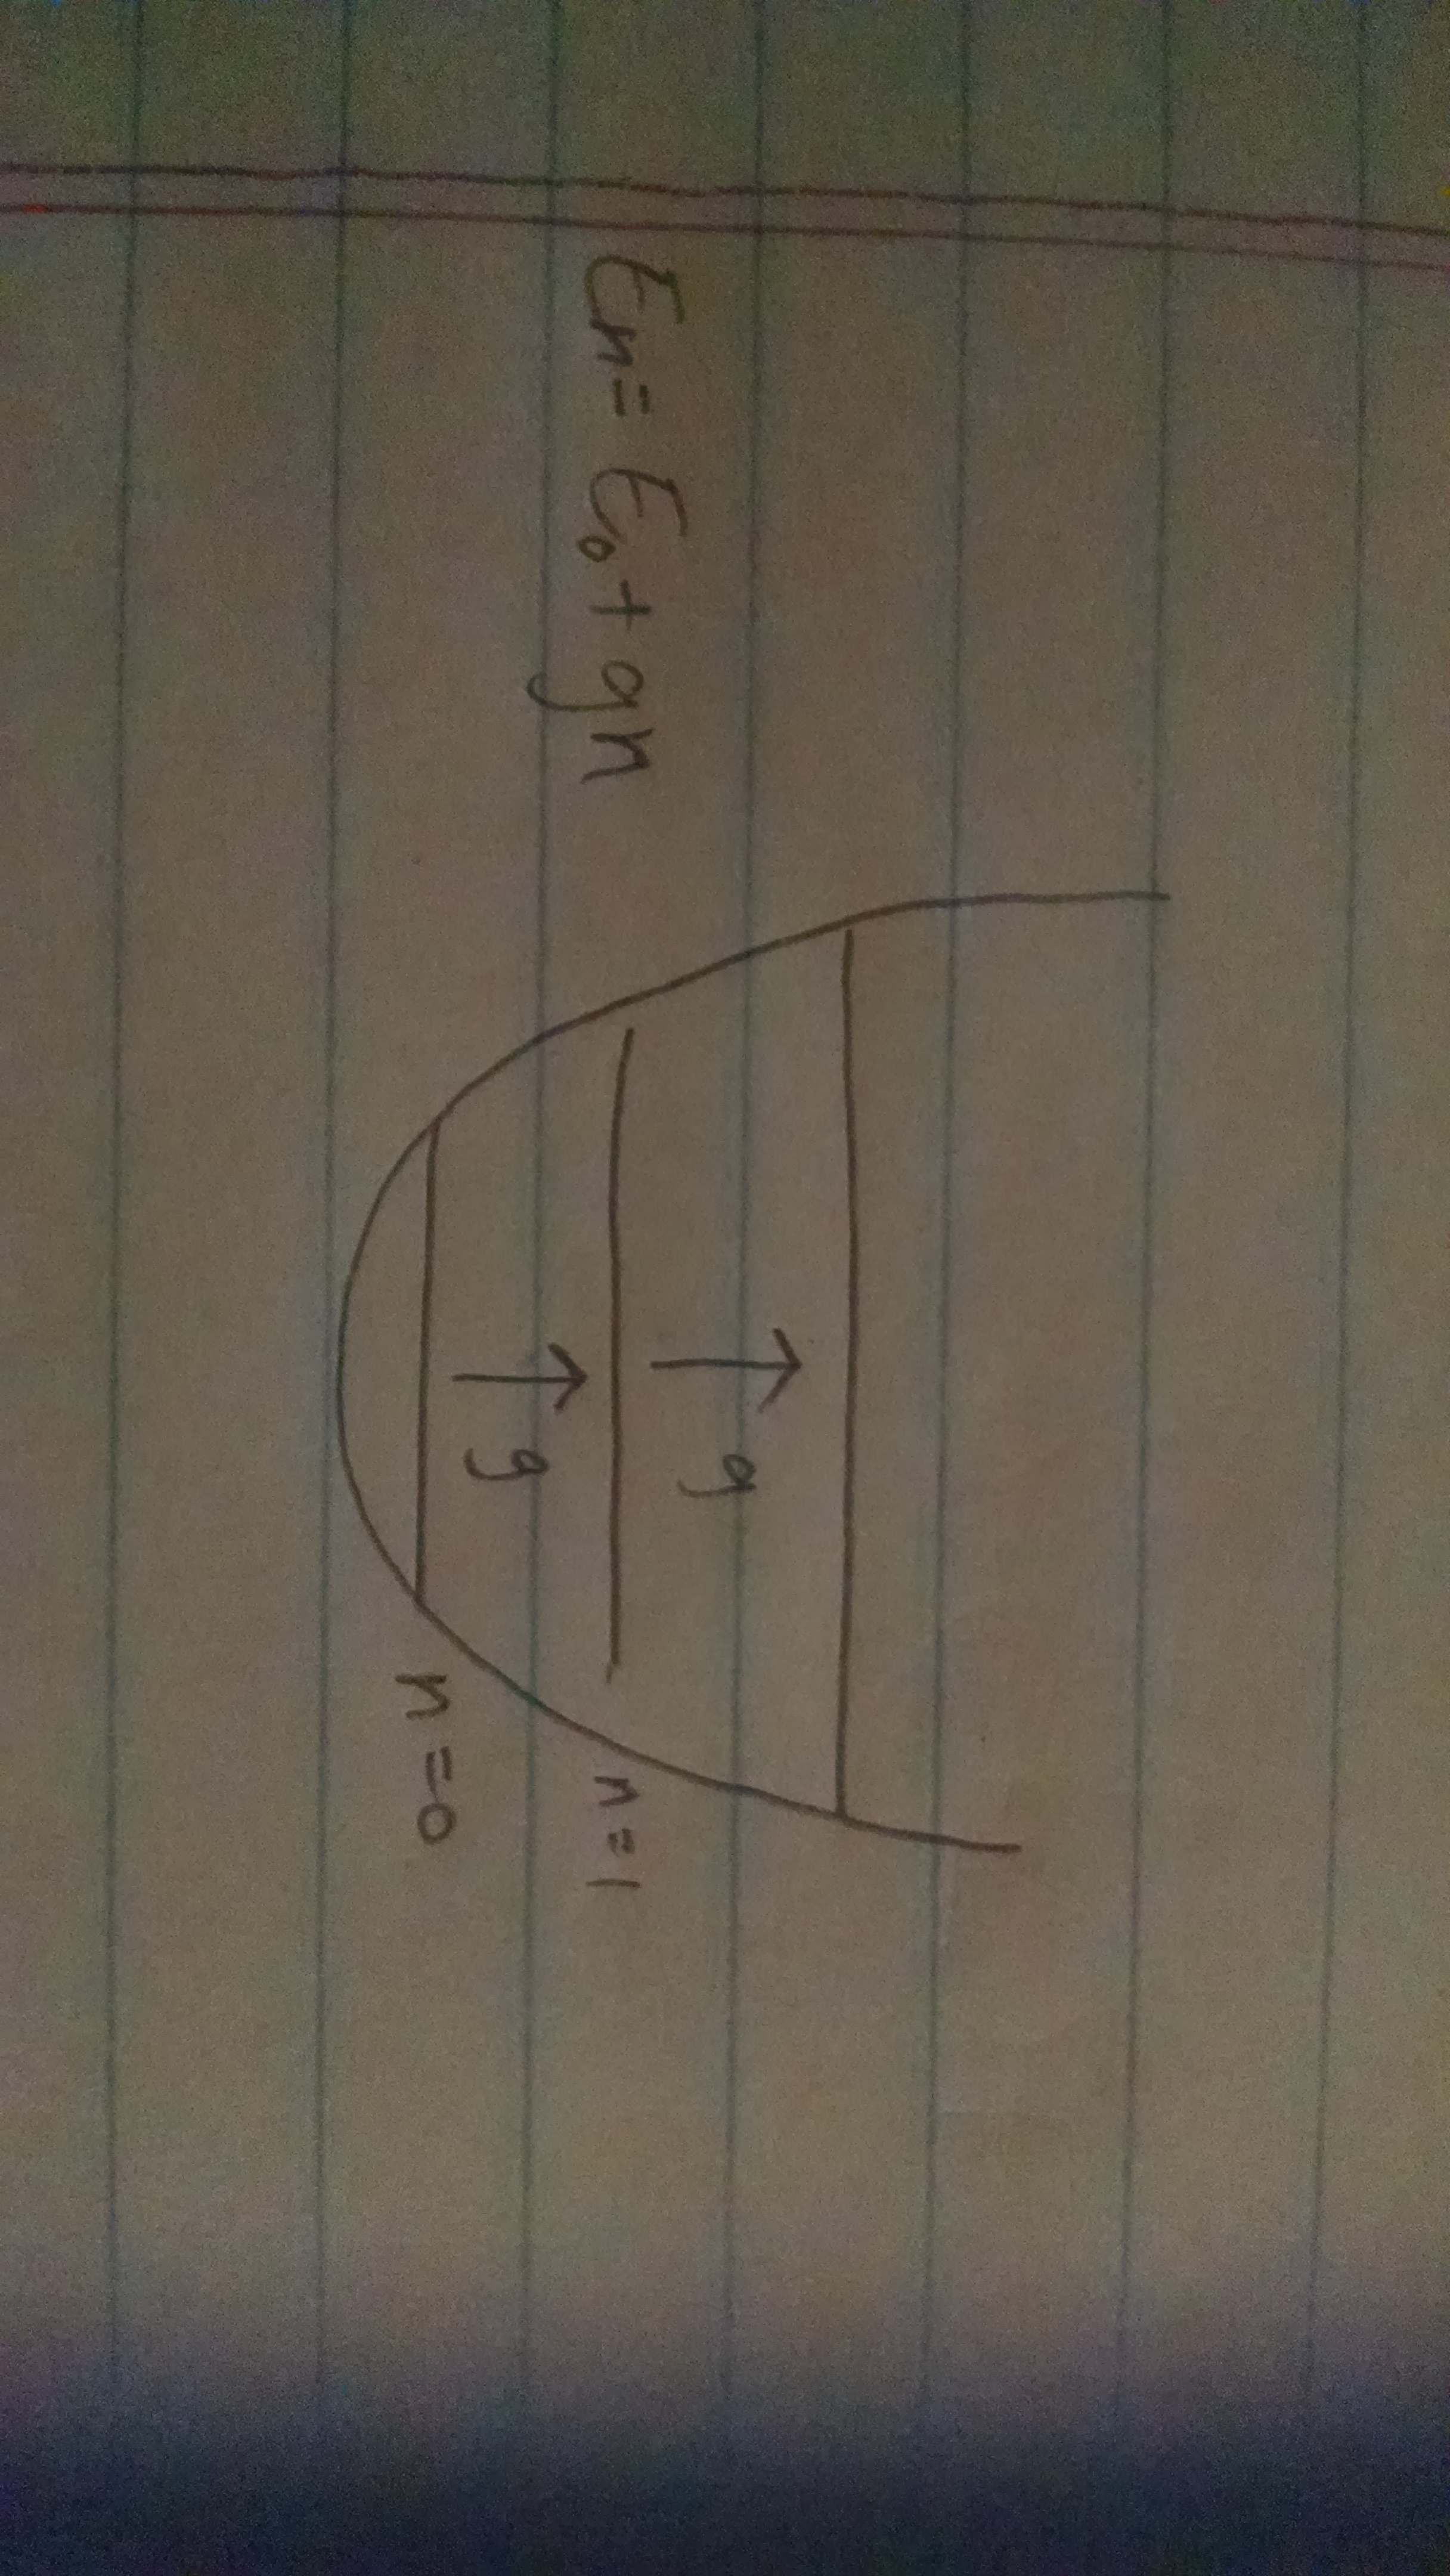
\includegraphics[scale=0.08,angle=90]{graphs2.jpg}
\end{figure}
\end{subanswer}
\end{answer}


\begin{answer}
10 Hours
\end{answer}

\begin{answer}
You know what would be nice? If we had bonus points or, alternatively, if we had some sort of mechanism for submitting assignments late. Thanks :)
\end{answer}
\end{document}